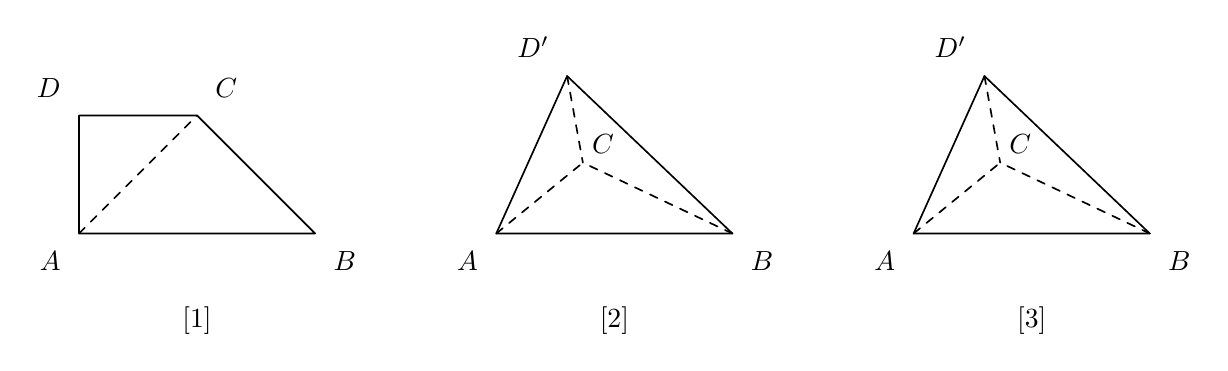
\begin{tikzpicture}[line width=0.6pt, line join=round, line cap=round, font=\normalsize]
  % panel 1: right trapezoid
  \begin{scope}[shift={(0,0)}]
    \coordinate (A) at (0,0);
    \coordinate (B) at (3.0,0);
    \coordinate (C) at (1.5,1.5);
    \coordinate (D) at (0,1.5);
    \draw (A) -- (B) -- (C) -- (D) -- cycle;
    \draw[dashed] (A) -- (C);
    \node[below left=3pt] at (A) {$A$};
    \node[below right=3pt] at (B) {$B$};
    \node[above right=3pt] at (C) {$C$};
    \node[above left=3pt] at (D) {$D$};
    \node at (1.5,-1.1) {\bitmapinsertcaption[1]};
  \end{scope}
  % panels 2 and 3: tetrahedra (same geometry)
  \begin{scope}[shift={(5.3,0)}]
    \coordinate (A) at (0,0);
    \coordinate (B) at (3.0,0);
    \coordinate (C) at (1.1,0.9);
    \coordinate (Dp) at (0.9,2.0);
    \draw (A) -- (B) -- (Dp) -- cycle;
    
    \draw[dashed] (A) -- (C);
    \draw[dashed] (B) -- (C);
    \draw[dashed] (Dp) -- (C);
    \node[below left=3pt] at (A) {$A$};
    \node[below right=3pt] at (B) {$B$};
    \node[above right=2pt,inner sep=1pt] at (C) {$C$};
    \node[above left=3pt] at (Dp) {$D'$};
    \node at (1.5,-1.1) {\bitmapinsertcaption[2]};
  \end{scope}
  \begin{scope}[shift={(10.6,0)}]
    \coordinate (A) at (0,0);
    \coordinate (B) at (3.0,0);
    \coordinate (C) at (1.1,0.9);
    \coordinate (Dp) at (0.9,2.0);
    \draw (A) -- (B) -- (Dp) -- cycle;
    
    \draw[dashed] (A) -- (C);
    \draw[dashed] (B) -- (C);
    \draw[dashed] (Dp) -- (C);
    \node[below left=3pt] at (A) {$A$};
    \node[below right=3pt] at (B) {$B$};
    \node[above right=2pt,inner sep=1pt] at (C) {$C$};
    \node[above left=3pt] at (Dp) {$D'$};
    \node at (1.5,-1.1) {\bitmapinsertcaption[3]};
  \end{scope}
\end{tikzpicture}
